\documentclass[]{article}
\usepackage{graphicx}
%opening
\title{ Report for Artificial Intelligence }
\author{ Simone D'Antimo, Francesco Caldivezzi, Harjot Singh}
\graphicspath{ {./images/} }

\begin{document}

\maketitle

\begin{abstract}
Coronavirus disease (COVID-19) has significantly affected the daily life activities of people globally.
To prevent the spread of COVID-19, the World Health Organization has recommended people to wear face masks in public places.
Manual inspection of people for wearing face masks in public places is a challenging task.  We deploy a
computer vision and deep learning framework to recognize if people wears or not mask.

The program we have implemented had 2 important parts: 
The first one is to recognize the face of a person, and to do that we use python with opencv libraries.

The second part of our project regards the model we use to estimate if a person is wearing a mask. We used the RES-Net 50V2 convolution neural network to create and train our model. Since the model created is very heavy we had to fine-tune it in order to implement it in our program.

The RES-Net 50 model that we created works really well with the dataset that we have used. We split data in 60 - 20 - 20 train-validation-test and the accuracy of the test set is 0.98.

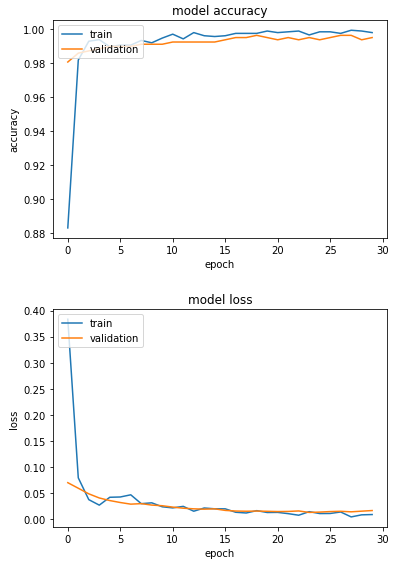
\includegraphics{LossAndAccuracy}

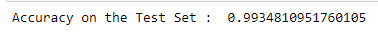
\includegraphics{testAccuracy}

roba usata per il crop dell'immagine, (?) 

conclusioni


Future works:
Since our model is heavy, also the fine-tuned one, it is possible that not all the device are able to compute it in a reasonable amount of time. In order to develop a program that may be used in a more heterogeneous amount of device we have found other models, thinner than Resnet50 V2, that may be implemented to scan face faster. This model is called MobileN.

Bibliography:

1) Face mask recognition system using CNN model https://www.sciencedirect.com/science/article/pii/S2772528621000352

2) A novel DeepMaskNet model for face mask detection and masked facial
recognition
 https://www.sciencedirect.com/science/article/pii/S1319157821003633

3) COVID-19 Face Mask Recognition with Advanced Face Cut Algorithm for Human Safety Measures https://arxiv.org/abs/2110.04316

4) Faster Region-based Convolutional Neural Network 
for Mask Face Detection 
https://ieeexplore.ieee.org/document/9651744

5) Mask wearing detection method based on SSD-Mask algorithm
https://ieeexplore.ieee.org/document/9443800

6) Face mask detection using deep learning: An approach to reduce risk of 
Coronavirus spread
https://www.sciencedirect.com/science/article/pii/S1532046421001775

7) The Face Mask Detection For Preventing the Spread 
of COVID-19 at Politeknik Negeri Batam
https://ieeexplore.ieee.org/document/9350556


\end{abstract}

\section{}

\end{document}
